\documentclass[12pt, titlepage]{article}
\usepackage{setspace}
\usepackage[letterpaper, margin=1in]{geometry}
\usepackage{booktabs}
\usepackage{tabularx}
\usepackage{graphicx}
\usepackage{nameref}
\usepackage{hyperref}

\title{SE 3XA3: Software Requirements Specification\\PyCards}
\author{Team 2,
		\\ Aravi Premachandran  premaa
		\\ Michael Lee  leemr2
		\\ Nikhil Patel  patelna2
}
\date{\today}

\newcommand {\PYVER}{2.7.xx }


\begin{document}
	\maketitle
	\pagenumbering{roman}
	\tableofcontents
	\listoftables
	\listoffigures
	\begin{table}[bp]
		\caption{\bf Revision History}
		\begin{tabularx}{\textwidth}{p{3cm}p{2cm}X}
			\toprule {\bf Date} & {\bf Version} & {\bf Notes}\\
			\midrule
			\mbox{October 11, 2016} & 1.0 & Initial Revision\\
			\mbox{October 30, 2016} & 1.1 & Revision 1\\
			\bottomrule
		\end{tabularx}
	\end{table}
	\newpage
	\pagenumbering{arabic}
	\section{Project Drivers}
		\subsection{The Purpose of the Project}
		\indent \indent PyCards is a collection of solitaire 
		(single-player) card games. It is designed to be a source of 
		entertainment for the end 
		user(s). The main objective for the product is to PyCards to be a 
		user-friendly application that our users can use to pass the time, have 
		fun, relax, and also challenge themselves.
		\subsection{The Stakeholders}
		\subsubsection{The Client}
		\indent \indent Our client is Dr. Smith, a professor at McMaster 
		University
		\subsubsection{The Customers}
		Our customer is any user who downloads and runs our program.
		\subsubsection{Other Stakeholders}
		Other stakeholders include the original developer of PySol, Markus 
		F.X.J. Oberhumer, as well as the many developers and contributors 
		PySolFC, the fork which we have based our program on.  In addition to 
		these, as the project is open source, the last group of stakeholders 
		are future contributors and developers to this software project.
	\subsection{Mandated Restraints}
		\subsubsection*{Constraint 1}  \label {constraint1}
		\indent The source code of the application shall be implemented 
		using the Python programming language, version \PYVER\\
		\textbf{Rationale 1}\\
		\indent The product should preserve compatibility for existing users of 
		the original implementation. The client should not be required to 
		upgrade or install new software in order to run the application.\\
		\textbf{Fit Criterion}\\
		\indent The product shall only require a Python interpreter 
		(and/or the inclusion of additional Python packages) in order to 
		operate. Exception will be made if either the entirety of the product 
		is ported to another language or if the necessary runtimes and 
		dependencies can be bundled with the product.\\\\
		
		\subsubsection*{Constraint 2} \label {constraint2}
		\indent The product shall be compatible with Windows operating systems 
		(Windows 10), Mac OSX, and Ubuntu provided that Python version \PYVER
		is compatible with the target system.\\
		\textbf{Rationale 2}\\
		\indent The client should not be required to migrate to newer (or 
		different) software or hardware in order to utilize the product.\\
		\textbf{Fit Criterion}\\
		\indent The product shall be tested on each of the specified systems by 
		the developers to ensure that it operates as expected and is fully 
		functional.\\\\
		
		\subsubsection*{Constraint 3} \label {constraint3}
		\indent The product shall be made available under the GNU GPLv3 or 
		later, along with any non-permissive terms added in accord with section 
		7 of the GNU GPLv3.\\
		\textbf {Rationale 3}\\
		\indent The original implementation was conveyed with this license and 
		as per 
		the conditions modified source versions must be licensed under the same 
		license.\\
		\textbf {Fit Criterion}\\
		\indent The product must adhere to the conditions of the GNU GPLv3 
		license.\\\\
		
		\subsubsection*{Constraint 4} \label {constraint4}
		\indent The source code for the product shall be publicly available but 
		the end product must also be deliverable as an standalone executable or 
		application for both Windows operating systems and Mac OSX operating 
		system.\\
		\textbf {Rationale 4}\\
		\indent The source code for the product must be publicly available as 
		per the conditions of the license. Users should not be required to be 
		familiar with the command-line/terminal in order to operate the 
		product.\\
		\textbf {Fit Criterion}\\
		\indent The final product should be available as a .exe executable for 
		Windows-based systems and as an application for OSX systems. The code 
		should be available in a publicly accessible repository.\\
		
		\subsection{Naming Conventions and Terminology}
		\textbf {API (Application Program Interface):} A set of routines, 
		protocols, and tools for interacting with a program\\
		\textbf {GNU GPLv3:} The GNU GPL (GNU General Public License)is a 
		software license, focused on freedom and free software.  Our software 
		project is licensed under version 3 of this license.  More information 
		on the terms and conditions of this license can be found at its 
		website: 
		\url{https://en.wikipedia.org/wiki/GNU_General_Public_License}\\
		\textbf {Free Software:} Software distributed under terms that allow 
		users to run the software for any purpose, as well as to study, change, 
		and distribute the software and any adapted versions.\\
		\textbf {PySolFC (PySol Fan Club Edition):} The program which our 
		project is based off of.\\
		\textbf {PySol:} The original program which PySolFC is based off of\\
		\textbf {Compatibility:} The ability of the product to operate on a 
		given
		\textbf{Klondike:} The most common solitaire game.  Most people think 
		of this variation when they think of solitaire, and it is the variation 
		included in the solitaire program found in older versions of Windows 
		(pre-windows 8).
		system. Full functionality is expected, unless otherwise specified, but
		performance, appearance, and other characteristics may vary\\
		\textbf {Implementation:} The object code, binaries, and/or executable form
		of the product, along with the source code used to create it\\
		\textbf {Product:} The entirety of the project, including but not limited to
		its source code, binaries, and documentation\\
		
		\subsection{Relevant Facts and Assumptions}
		
		\textbf{Relevant Facts}
		\vspace{-2mm}
		\begin{itemize}
			\itemsep0em
			\item The existing implementation is implemented purely in 
			the Python programming language.
			\item Mac OSX and Ubuntu come with a Python environment 
			pre-installed. The installed version may or may not be compatible 
			with 
			the product.
		\end{itemize}
		\textbf{Assumptions}
		\vspace{-2mm}
		\begin{itemize}
			\itemsep0em
			\item 	It is not feasible for the product to be tested for 
			compatibility on all of the various operating systems. As such it 
			will only be tested on the latest version of each major operating 
			system as previously specified.
			\item The product assumes that the system that it will be operated 
			on includes peripherals such as a mouse, keyboard and display.
		\end{itemize}
		
	\section{Functional Requirements}
		\subsection{The Scope of the Work and the Product}
		%\subsection{The Current Situation}
		%\indent There already exists an implementation that has a similar 
		%purpose as that of our product, namely PySol Fan Club Edition. This 
		%implementation was coded entirely in Python and is an open-source 
		%software product.\\
		\subsubsection{The Context of the Work}
		\indent Our product shall be based upon the implementation PySol Fan Club
		Edition however it shall be redeveloped in order to satisfy the constraints
		and requirements defined in this document.\\
		\subsubsection{Work Partitioning}
		\begin{table}[!htp]
		\caption{\bf Work Partitioning}
			\begin{tabularx}{\textwidth}{|l|X|X|}
			\toprule {\bf Event Name} & {\bf Input/Output} & {\bf Summary}\\
			\midrule			
			\mbox{User changes game} & Game ID(IN) & The user selects a different game.
			The system prompts for confirmation to discard the current game. The system
			destroys the current game and creates the new game\\
			\hline
			\mbox{User changes background} & File Path(IN) \newline or Color(IN) & 
			The user selects a new background image from the file system or chooses
			a solid color to use. The system redraws the window with the new color\\
			\hline
			\mbox{User changes cardset} & File Path(IN) & The user selects the new
			cardset to use. The system attempts to load the cardset and then redraws the
			game using the new cardset images\\
			\hline
			\mbox{User selects a card} & ButtonPress(IN) & The user clicks on a card. The
			system checks if the selection is valid and then highlights and tracks the
			cursor with the selected card(s)\\
			\bottomrule
			\end{tabularx}
		\end{table}
		\subsubsection{Individual Product Use Cases}
		\begin{figure}[h!]
			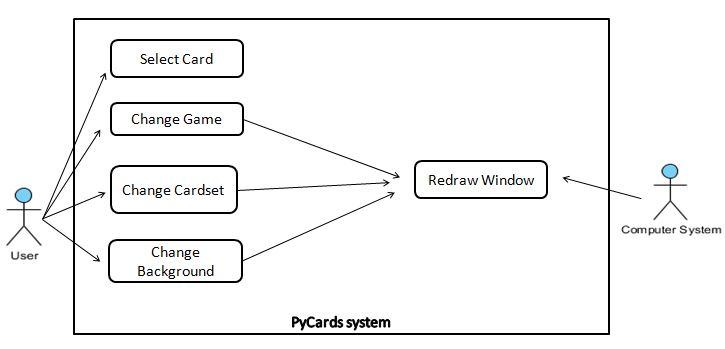
\includegraphics[scale=0.9]{use_case}
			\caption{Use Case Diagram for PyCards}
			\label{usecase}
		\end{figure}
		\subsection{Functional Requirements}
		\indent \indent \textbf {Functional Requirement 1} \label{freq1}\\
		\indent \indent The program will be executed on a computer compatible with
		Python version \PYVER\\
		\indent \textbf {Fit Criterion}\\
		\indent \indent The functionality of the program on the major operating
		systems - Windows 10, Ubuntu, Mac OSX - will be tested before release\\\\
		\indent \textbf {Functional Requirement 2} \label{freq2}\\
		\indent \indent The program will execute in its own graphical window\\
		\indent \textbf {Fit Criterion}\\
		\indent \indent Check that the graphical user interface is successfully
		created and fully functional on the target system(s).\\\\
		\indent \textbf {Functional Requirement 3} \label{freq3}\\
		\indent \indent The user’s game statistics will persist even after the 
		application is	terminated\\
		\indent \textbf {Fit Criterion}\\
		\indent \indent Upon re-launching the application the player statistics will
		correspond to the statistics present when the application was most recently
		terminated.\\\\
		\indent \textbf {Functional Requirement 4} \label{freq4}\\
		\indent \indent The program shall provide the user with the option to start a 
		new game\\
		\indent \textbf {Fit Criterion}\\
		\indent \indent The user interface should contain a button that when pressed 
		will trigger the start of a new game.\\\\
		\indent \textbf{Game Aspect Specific Requirements:} \label{GASR}
		\vspace{-2mm}
		\begin{itemize}
			\itemsep0em
			\item The program shall provide users with the ability to start new 
			games, save games, and load already saved games.
			\item The program shall provide users with an interface to 
			customize the game window, namely the background and cardset to be 
			used.
			\item The program shall adhere to the rules of the game in progress
			\item Upon completion of a game, the user shall be prompted to 
			start a new game
		\end{itemize}
		\indent \textbf{Klondike Requirements:} \label{Kreq}
		\vspace{-2mm}
		\begin{itemize}
			\itemsep0em
			\item The playing cards are organized into NUM\_DECKS deck stack, 
			NUM\_WASTES waste stack, NUM\_FOUNDATIONS foundation stacks and 
			NUM\_NORMAL\_STACKS alternating-colour stacks
			\item Cards cannot be added to the deck or waste stack(s) by the 
			player
			\item The waste stack(s) can be recycled to the deck stack 
			NUM\_REDEAL times
			\item If the player clicks on the deck stack, the top BURN\_NUM 
			cards from the deck stack will be moved to the waste stack
			\item The player can only select and move the current top card from 
			the waste stack
			\item The foundation stacks are initially empty.
			\item The player can build the foundation stacks by placing on it 
			cards of the same suit in order of increasing rank 
			(FOUNDATION\_BASE to King). These cards must be placed one at a time.
			\item If the player successfully builds all four foundation stacks 
			(to King) then (s)he wins the game and a dialogue is shown 
			confirming the successful completion of the game.
			\item The player can build the alternating-suit stacks by forming 
			stacks of cards of opposite colours and decreasing (by 1) rank
			\item Multiple cards in the same stack can be moved at the same 
			time provided that sequence of cards to be moved is alternating in 
			colour and the rank of each subsequent card is one lower than that 
			of the previous card (with the exception of the first card at the 
			bottom of the stack of selected cards which has no previous)
			\item If an alternating-suit stack is empty, only sequences 
			starting with STACK\_BASE can be moved to it
			\item If as a result of moving cards, the top card of a stack is 
			face-down, that card is then flipped over to become face-up
		\end{itemize}
	
	\section{Non-functional Requirements}
		\subsection{Look and Feel Requirements}
		\begin{itemize}
			\itemsep0em
			\item The product shall represent cards with images of playing 
			cards and additional areas that can be interacted with (ex. where 
			cards can be placed) shall be outlined for the user to see.
		\end{itemize}
		\subsection{Usability and Humanity Requirements}
		\begin{itemize}
			\itemsep0em
			\item The product shall be easy for a child with basic reading and 
			computer abilities to use
		\end{itemize}
		\subsection{Performance Requirements}
		\begin{itemize}
			\itemsep0em
			\item Normal interaction actions with the game shall take no longer 
			than if an average user were playing the same game with a physical 
			deck of cards.
		\end{itemize}
		\subsection{Operational and Environmental Requirements}
		\begin{itemize}
			\itemsep0em
			\item Users will interact with the product using a mouse and 
			keyboard connected to their computer
		\end{itemize}
		\subsection{Installability Requirements}
		\begin{itemize}
			\itemsep0em
			\item The game will not need to be installed to the user's device; instead
			it will be packaged and self-contained, runnable as a portable application.
		\end{itemize}
		\subsection{Maintainability and Support Requirements}
		\begin{itemize}
			\itemsep0em
			\item The product is expected to run on Windows 10, Mac OSX, and 
			Ubuntu systems that have Python version \PYVER installed.
		\end{itemize}
		\subsection{Security Requirements}
		\begin{itemize}
			\itemsep0em
			\item The source code for the product is publicly available and as such
			anyone can download, modify, and produce modified version of the project.
			However, only the developer team is allowed to directly make changes to the 
			repository
			\item When the product is made ready for distribution, the packaged product
			shall have a checksum (ie. MD5 checksum) for verifying authenticity
		\end{itemize}
		\subsection{Cultural Requirements}
		\begin{itemize}
			\itemsep0em
			\item The product will not contain images or text that would be 
			considered offensive.
		\end{itemize}
		\subsection{Legal Requirements}
		\begin{itemize}
			\itemsep0em
			\item The product is licensed under the  GPLv3 license and must 
			conform to the license and any non-permissive terms added in 
			accordance to section 7 of the GNU GPLv3 license.
		\end{itemize}
		\subsection{Health and Safety Requirements}
		\begin{itemize}
			\itemsep0em
			\item This product requires the use of a pointing device and that the user
			views and interacts with a graphical user interface. Excessive use of this
			product may cause strain or injury including but not limited to eye strain
			and injury to arms, wrists, and/or hands including carpal tunnel syndrome.
		\end{itemize}
		
	\section{Project Issues}
		\subsection{Open Issues}
		\begin{itemize}
		\itemsep0em	
			\item The main open issue is the possibility of the graphics extension
			provided by the open source project being incompatible. Seeing as the team
			has permission to use and modify the existing implementation, many of the
			issues a new project would face have been accounted for
			\item Python includes a lot of built-in libraries that will be used in the
			 implementation. One such library is Tkinter, used for the graphical portion
			of the product
			\item The existing implementation PySolFC is an off-the-shelf solution,
			and so is the project that PySolFC was based upon, the original PySol
		\end{itemize}
		\subsection{New Problems}
		\begin{itemize}
		\itemsep0em	
			\item Any changes to the original Tkinter graphics library or the 
			custom interfaces that PySolFC provides to the library could make it
			incompatible with our reimplementation and would thusly affect the work of
			our developer team. It would require the adaptation of our code to the new
			API which could introduce problems
			\item The program should not require a lot of RAM when it’s running or
			have high disk usage or requirements of the user’s system. Overall the
			project should not have overly high resource consumption on the target system\\
		\end{itemize}
		\subsection{Tasks}
			\indent The team plan on completing this project by completing the problem
			statement and requirements documents before beginning programming. With these
			documents the team will have a strong understanding of what needs to done.
			From then onwards developers will work on implementing the program using
			the Model View Controller software architecture and referring to the existing
			project if and when needed. To manage the project we’ll be using version
			control via git.\\


		\subsection{Migration to the New Product}
			\indent There are no major requirements for migration as we intend to
			distribute the program as a standalone executable (while making the source
			available to interested parties). As such the product will be able to coexist
			with the existing products PySol and PySolFC. Furthermore, packaging
			or bundling as an executable (or application) allows the product to be
			self-contained with minimal external dependencies.\\
			\indent The existing implementation however, if installed, adds its modules
			to the python directory for 3rd party packages. Facilitating its removal
			would require us to reverse that modification and by removing or updating
			the specified files\\

		\subsection{Risks}
		\begin{itemize}
			\itemsep0em
			\item Excessive pressure due to time constraints for deliverables
			\item Inaccurate quantification of objectives
			\item Inadequate testing of graphical user interface
		\end{itemize}

		\subsection{Costs}
			\indent The product being developed is open-source as is the implementation
			it is based upon. To follow and propagate the concept of open-source
			software, only freely available software shall be used in the development
			process.\\
			\indent The primary and only significant cost of the project to date is the
			time and effort spent by its developers. The cost is anticipated to be around
			5 hours or more of time spent per person per week for the duration of
			September-December 2016.\\

		\subsection{User Documentation and Training}
			\indent In-person training will not be required and therefore will not be
			provided for this product. However, user documentation will be included with
			the packaged product. A specifications document including APIs, modular
			decomposition, and also build and modification instructions shall accompany
			the source for the product.\\
	 		\indent The user documentation shall provide enough guidance that a user
			with no previous exposure to the product shall after reading be able to
			achieve basic objectives. These objectives include but are not limited to
			navigating the interface, starting a new game, and accessing the demo
			feature.\\
	 		\indent The user documentation shall include a section (or multiple
			sections) that display the rules of the available games.

		\subsection{Waiting Room}		
		\indent Some possible requirements we could address if time permits:\\
		\begin{itemize}
			\itemsep0em
			\item Create more games (version 1.1)\\
			By creating more games users will have more options and be less likely to
			become bored or disinterested
			\item Improve the graphics (version 1.1) \\
			By improving the graphics, the program will avoid the risk of seeming
			outdated or becoming obsolete
			\item Create a leaderboard (version 1.2)\\
			By creating a leaderboard, it will keep people more engaged and bring out
			their competitiveness which will motivate them to use the product more
		\end{itemize}		
		\subsection{Ideas for Solutions}
		
	\newpage
	\section{Appendix}
	\subsection{Symbolic Parameters}
		\begin{itemize}
			\itemsep0em
			\item NUM\_REDEALS = Unlimited
			\item FOUNDATION\_BASE = Ace
			\item STACK\_BASE = King
			\item NUM\_DECKS = 1
			\item NUM\_WASTES = 1
			\item NUM\_FOUNDATIONS = NUM\_SUITS = 4
			\item NUM\_NORMAL\_STACKS = 7
		\end{itemize}

\end{document}

